\begin{flushright} {\tiny {\color{gray} (tikz\_quadrature\_both.tex)}} \end{flushright}
%~~~~~~~~~~~~~~~~~~~~~~~~~~~~~~~~~~~~~~~~~~~~~~~~~~~~~~~~~~~~~~~~~~~~~~~~~~~~~~~~~~~~~~~~~~~~~~~~~~

\begin{center}
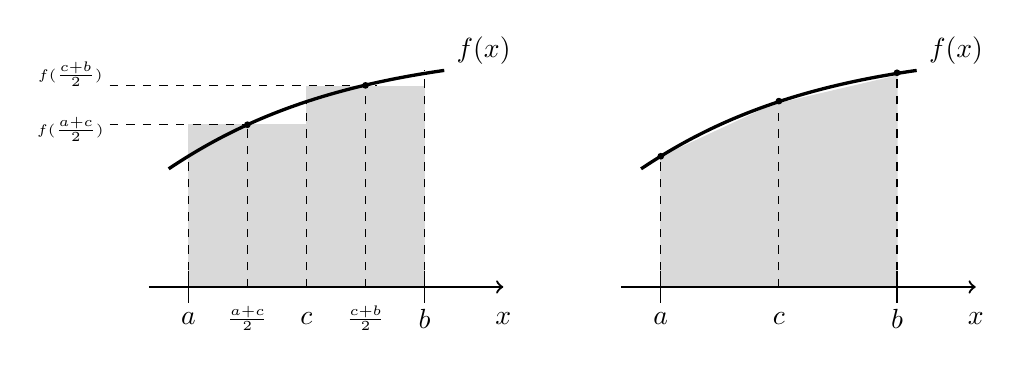
\begin{tikzpicture}
%\draw[step=0.5cm,gray,very thin] (0,0) grid (12,5); 
\draw[fill=gray!30,gray!30](1,1) rectangle (2.5,3.06);
\draw[fill=gray!30,gray!30](2.5,1) rectangle (4,3.55);
\draw [thick, ->] (0.5,1) -- (5,1);
\node[] at (1,0.6) {$a$};
\node[] at (4,0.6) {$b$};
\node[] at (5,0.6) {$x$};
\node[] at (2.5,0.6) {$c$};
\node[] at (1.75,0.6) {\tiny $\frac{a+c}{2}$};
\node[] at (3.25,0.6) {\tiny $\frac{c+b}{2}$};
\draw [-] (1,0.8) -- (1,1.2);
\draw [-] (4,0.8) -- (4,1.2);
\draw [dashed] (1,1) -- (1,2.6);
\draw [dashed] (2.5,1) -- (2.5,3.35);
\draw [dashed] (4,1) -- (4,3.75);
\draw [dashed] (1.75,1) -- (1.75,3.06);
\draw [dashed] (3.25,1) -- (3.25,3.56);
\draw[black,fill=black] (1.75,3.06)  circle (1pt);
\draw[black,fill=black] (3.25,3.56)  circle (1pt);
\draw[very thick] (0.75,2.5) .. controls (1.5,3) and (2.5,3.5) .. (4.25,3.75);
\node[] at (4.75,4) {$f(x)$};
\node[] at (-0.5,3.) {\tiny $f(\frac{a+c}{2})$};
\draw [dashed] (0,3.06) -- (1.75,3.06);
\node[] at (-0.5,3.7) {\tiny $f(\frac{c+b}{2})$};
\draw [dashed] (0,3.56) -- (3.4,3.56);

%------------------------------------------------

\draw[fill=gray!30,gray!30] (7,1)--(8.5,1)--(8.5,3.35)--(7,2.65)--cycle;
\draw[fill=gray!30,gray!30] (8.5,1)--(10,1)--(10,3.68)--(8.5,3.33)--cycle;
\draw [thick, ->] (6.5,1) -- (11,1);
\node[] at (7,0.6) {$a$};
\node[] at (10,0.6) {$b$};
\node[] at (11,0.6) {$x$};
\node[] at (8.5,0.6) {$c$};
\draw [-] (7,0.8) -- (7,1.2);
\draw [-] (10,0.8) -- (10,1.2);
\draw [dashed] (7,1) -- (7,2.6);
\draw [dashed] (8.5,1) -- (8.5,3.35);
\draw [dashed] (10,1) -- (10,3.75);
\draw[very thick] (6.75,2.5) .. controls (7.5,3) and (8.5,3.5) .. (10.25,3.75);
\node[] at (10.75,4) {$f(x)$};
\draw[black,fill=black] (7,2.66)  circle (1pt);
\draw[black,fill=black] (8.5,3.36)  circle (1pt);
\draw[black,fill=black] (10,3.72)  circle (1pt);
\end{tikzpicture}
\end{center}

